% Figure 3.1 (dlsu-manuscript/chapter_3.tex, fig:conceptual), unchanged except for font and colors.
\documentclass[12pt,border=10pt]{standalone}
% Shared style for the slide figures: sans-serif text (Helvetica, close to the Arial of the charts),
% the same colors as charts.py, and the manuscript's table tools.
\usepackage[T1]{fontenc}
\usepackage[scaled]{helvet}
\renewcommand{\familydefault}{\sfdefault}
\usepackage{amsmath,amssymb}
\usepackage{sansmath}
\usepackage{xcolor}
\usepackage{booktabs,array}
\newcolumntype{L}[1]{>{\raggedright\arraybackslash}p{#1}}
\usepackage{tikz}
\usetikzlibrary{arrows.meta,positioning,calc}

\definecolor{ink}{HTML}{0B0B0B}
\definecolor{inktwo}{HTML}{52514E}
\definecolor{muted}{HTML}{898781}
\definecolor{gridc}{HTML}{E1E0D9}
\definecolor{basec}{HTML}{C3C2B7}
% one color per selection rule, in the fixed categorical order of the charts
\definecolor{cp}{HTML}{2A78D6}     % k-Changepoint (content)
\definecolor{sme}{HTML}{EB6834}    % SME (position)
\definecolor{posc}{HTML}{1BAF7A}    % positional (position)
\definecolor{rnd}{HTML}{EDA100}    % random (chance)
\definecolor{bocpd}{HTML}{E87BA4}  % k-BOCPD (content), categorical slot 5
\definecolor{temporal}{HTML}{6250D6}  % temporal information added to the mean (frame combinations figure)

\newcommand{\chip}[1]{\tikz[baseline=0.1ex]\fill[#1, rounded corners=1pt] (0,0) rectangle (0.32cm,0.32cm);}
\AtBeginDocument{\sansmath\color{ink}}
\hyphenpenalty=10000 \exhyphenpenalty=10000   % no hyphenated words on slides

\begin{document}
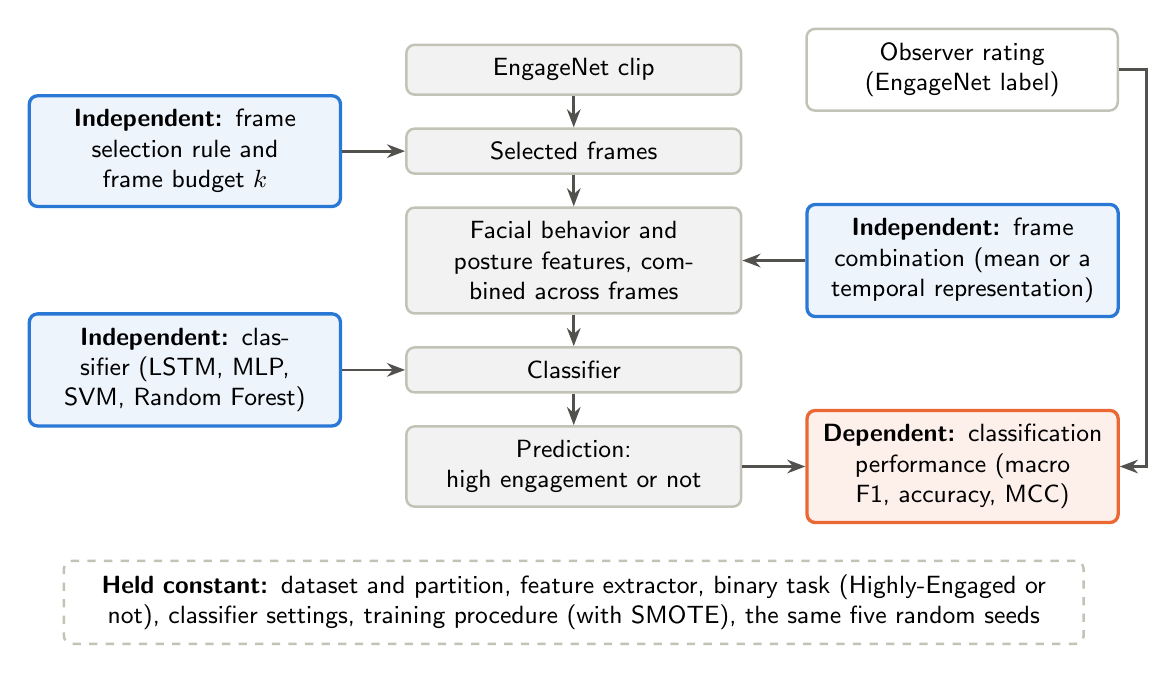
\begin{tikzpicture}[
   node distance=0.4cm,
   chainbox/.style={draw=basec, line width=0.9pt, rounded corners=3pt, align=center, text width=3.9cm, inner sep=5pt, font=\small, fill=black!5},
   var/.style={draw=cp, line width=1.2pt, fill=cp!8, rounded corners=3pt, align=center, text width=3.6cm, inner sep=5pt, font=\small},
   plain/.style={var, draw=basec, fill=white, line width=0.9pt},
   arr/.style={-{Stealth[length=2.3mm]}, line width=1pt, color=inktwo}
]
   \node[chainbox] (clip) {EngageNet clip};
   \node[chainbox, below=of clip] (frames) {Selected frames};
   \node[chainbox, below=of frames] (feat) {Facial behavior and posture features, combined across frames};
   \node[chainbox, below=of feat] (clf) {Classifier};
   \node[chainbox, below=of clf] (pred) {Prediction:\\high engagement or not};

   \node[var, left=0.8cm of frames] (rule) {\textbf{Independent:} frame selection rule and frame budget $k$};
   \node[var, left=0.8cm of clf] (model) {\textbf{Independent:} classifier (LSTM, MLP, SVM, Random Forest)};
   \node[var, right=0.8cm of feat] (combo) {\textbf{Independent:} frame combination (mean or a temporal representation)};
   \node[plain, right=0.8cm of clip] (label) {Observer rating (EngageNet label)};
   \node[var, draw=sme, fill=sme!10, right=0.8cm of pred] (perf) {\textbf{Dependent:} classification performance (macro F1, accuracy, MCC)};

   \node[draw=basec, dashed, line width=0.9pt, rounded corners=3pt, align=center, text width=12.6cm, inner sep=5pt, font=\small, anchor=north] (const)
      at ([yshift=-0.45cm]perf.south -| pred.south) {\textbf{Held constant:} dataset and partition, feature extractor, binary task (Highly-Engaged or not), classifier settings, training procedure (with SMOTE), the same five random seeds};

   \draw[arr] (clip) -- (frames);
   \draw[arr] (frames) -- (feat);
   \draw[arr] (feat) -- (clf);
   \draw[arr] (clf) -- (pred);
   \draw[arr] (rule) -- (frames);
   \draw[arr] (combo) -- (feat);
   \draw[arr] (model) -- (clf);
   \draw[arr] (pred) -- (perf);
   \draw[arr] (label.east) -- ++(0.35,0) |- (perf.east);
\end{tikzpicture}
\end{document}
